%!TEX root = ../../main.tex

\section{Transcending the DAP}

\subsection{Custom Events and Commands}%
\label{sec:dap-custom}

As stated at various points, the main restriction of the current debugger is
strict adherence to the confines of the Debug Adapter Protocol. Despite the DAP
being supplied with a finite set of commands, both the DAP library used in
Gillian and the debugger extension API in Visual Studio Code support the use of
custom commands and extensions%
~\cite{ocaml-dap-custom, vscode-dap-custom-event, vscode-dap-custom-request}, as
outlined in \autoref{sec:vscode}.

As an introduction to working with DAP extensions, the custom \texttt{log} event
was introduced (\autoref{lst:custom-log-event}). Since running Gillian in
debugging mode has standard output captured as the primary form of communication
with the IDE, direct console printing is no longer a possibility. This event
can be used a replacement, requesting that the IDE logs the relevant message.
This has the added benefit of allowing arbitrary JSON to be passed as well,
where many IDEs present logged JSON in a pretty and collapsible format
(\autoref{fig:log-json}).

\begin{listing}[!ht]
\noindent\rule{\textwidth}{0.5pt}
\vspace{-0.6cm}
\begin{minted}{ocaml}
module Log_event = struct
  let type_ = "log"

  module Payload = struct
    type t = { msg : string; json : JsonMap.t }
    [@@deriving yojson { strict = false }]
  end
end
\end{minted}
\vspace{-0.4cm}
\noindent\rule{\textwidth}{0.5pt}
\vspace{-0.6cm}
\caption{The custom \texttt{log} event, in \texttt{Debugger\_log.ml}}
\label{lst:custom-log-event}
\end{listing}

\begin{figure}
  \center{}
  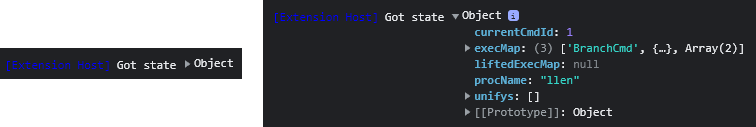
\includegraphics[width=0.6\textwidth]{img/log-json.png}
  \caption{
    The result of emitting a \texttt{log} event, with a collapsed (left) and
    expanded (right) JSON object}%
  \label{fig:log-json}
\end{figure}

And with that, Gillian's debug adapter was ready to be extended. The newly added
events and commands, contained in \texttt{dapCustom.ml}, consist of:
\begin{itemize}
  \item \texttt{Debug\_state\_update\_event} --- automatically sent alongside
        the \texttt{Stopped\_event}, providing some information on the current
        state of the debugger (\autoref{lst:debugstate})
  \item \texttt{Debugger\_state\_command} --- responds with the same debugger
        state information as\newline\texttt{Debug\_state\_update\_event}
  \item \texttt{Unification\_command} --- gives information on the unification
        at the specified report ID, should one exist
  \item \texttt{Jump\_command} --- instructs the debugger to `jump' to the
        command at the specified report ID, travelling forwards or backwards
        (or sideways) in time
  \item \texttt{Step\_specific\_command} --- jumps to the specified ID, as with
        the \texttt{Jump\_command}, but also executes a symbolic step at the
        (optionally) specified branch case; this directly makes use of the
        branch-aware interpreter introduced in
        \autoref{sec:interpreter-branching}
\end{itemize}

\begin{listing}[!ht]
\noindent\rule{\textwidth}{0.5pt}
\vspace{-0.6cm}
\begin{minted}{ocaml}
type debug_state = {
  exec_map : exec_map_pkg; [@key "execMap"]
  lifted_exec_map : exec_map_pkg option; [@key "liftedExecMap"]
  current_cmd_id : rid; [@key "currentCmdId"]
  unifys : (rid * Unifier.unify_kind * UnifyMap.unify_result) list;
  proc_name : string; [@key "procName"]
}
[@@deriving yojson]
\end{minted}
\vspace{-0.4cm}
\noindent\rule{\textwidth}{0.5pt}
\vspace{-0.6cm}
\caption{The \texttt{debug\_state} type, of \texttt{Debugger.Inspect}}
\label{lst:debugstate}
\end{listing}


\subsection{A Rich Debugging Interface}%
\label{sec:debug-interface}

With the debug adapter extensions in place, focus shifted from development of
the Gillian program itself to an extension for Visual Studio Code. The extension
code provided in a project last year~\cite{gillian-debugging-2021} formed a
solid foundation, providing all the boilerplate necessary to instruct VSCode to
use Gillian as a debugger. However, for the extension required, the debug API
is only one half of the coin; to create a bespoke user interface for Gillian
debugging, the best course of action was to use a webview.

Working with a webview was a first for this project, regarding the history of
Gillian. As there existed no baseline code to iterate on, some research was
performed to find the best practices, or at least clean examples of the kind
of solution required. The decision was made to develop the webview UI using
React; while the use of React, or any other fully-featured frontend framework,
was quite unconventional in the context of webviews, research led to the
discovery of a UI toolkit for working in React webviews, including a variety
of React components~\cite{vscode-ui-toolkit}. In an article about the discovery
of this toolkit~\cite{vscode-ui-toolkit-article}, the motivation for such was
revealed to be a VSCode extension that makes use of a custom webview UI, with
React; precisely the kind of setup that Gillian was in need of. This extension,
`Flat Editor'~\cite{flat-editor}, provided all the boilerplate needed to set
Gillian up with a React-enabled webview of its very own, including TypeScript
for static type checking and PostCSS for convenient CSS processing at build
time.

\begin{figure}
  \center{}
  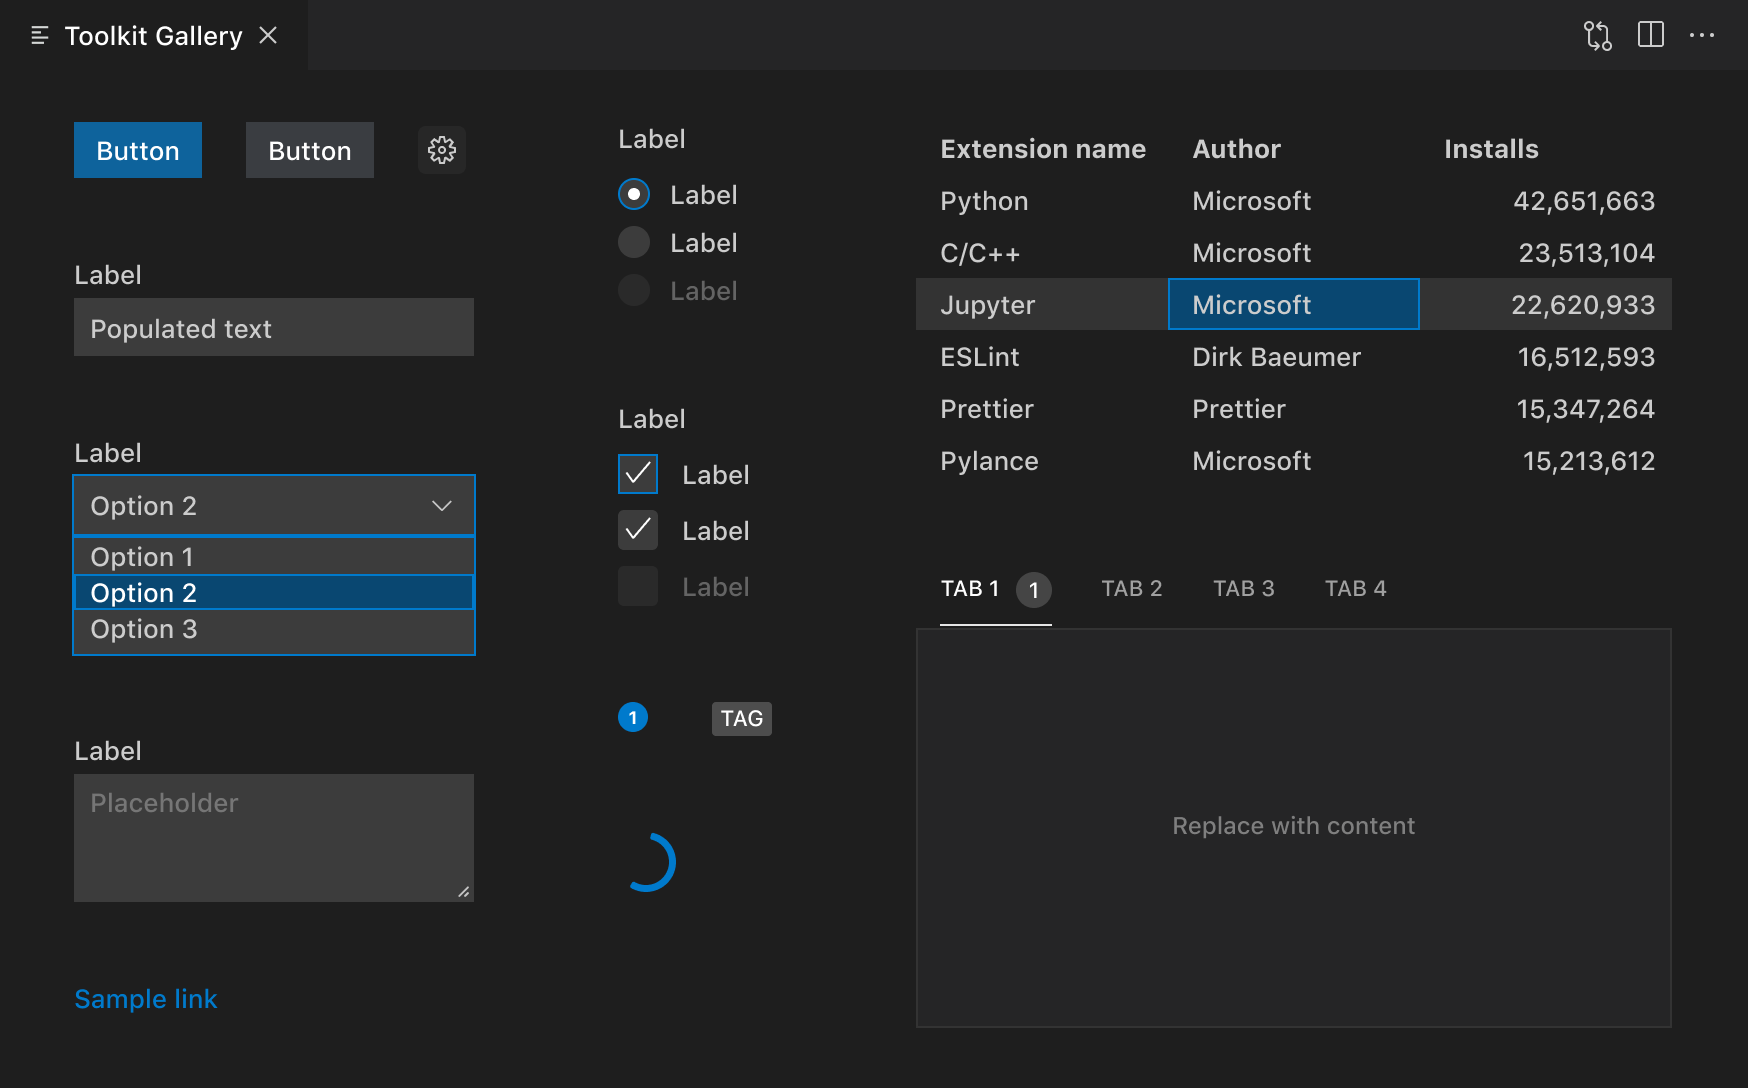
\includegraphics[width=0.8\textwidth]{img/vscode-ui-toolkit-demo.png}
  \caption{
    A demonstration of the components made available by the VSCode UI toolkit,
    from~\cite{vscode-ui-toolkit}}%
  \label{fig:vscode-ui-toolkit-demo}
\end{figure}

Now that the webview boilerplate was in place, it was time to start building the
UI.\@ The first hurdle to this process was finding a way to elegantly render
the execution tree; ultimately, React Flow~\cite{react-flow} was settled upon,
providing an excellent amount of customisability, at the sacrifice of requiring
more involvement in its configuration. It also has the benefit of providing,
out of the box, a pannable, zoomable viewport for the rendered tree.

\begin{figure}
  \center{}
  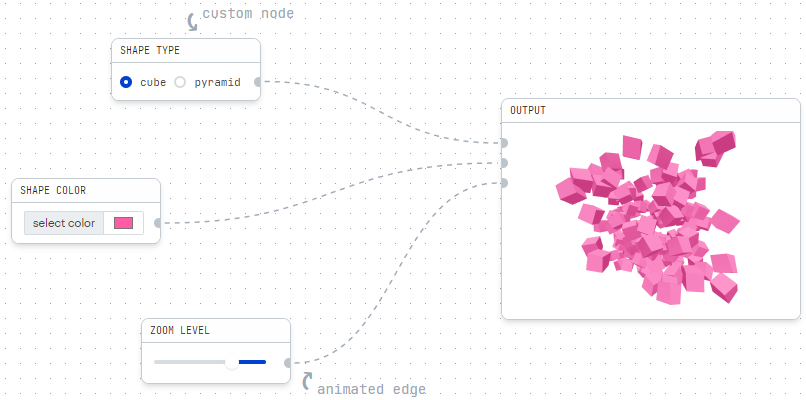
\includegraphics[width=0.8\textwidth]{img/react-flow-demo.png}
  \caption{
    A demonstration of the React Flow's capabilities,
    from~\cite{react-flow}}%
  \label{fig:react-flow}
\end{figure}

The first component developed for the UI was the execution map, whose
prerequisites were twofold; a mechanism for transforming an \texttt{ExecMap}
into a list of nodes suitable for React Flow and the edges that connect them,
and a React component to render those nodes in a clear and elegant manner. The
first iteration of the exec map view, shown in \autoref{fig:execmap-init},
displays distinct paths of execution, while clearly denoting the current
command. Each command node has a button that triggers a \texttt{Jump\_command}
for the relevant command ID, and a command that has yet to be executed, denoted
by the circular, dotted node, similarly triggers a
\texttt{Step\_specific\_command}.

A fortunate consequence of using the VSCode UI toolkit, along with using the CSS
variables provided by VSCode for styling~\cite{vscode-theme}, is the interface's
ability to instantly adapt to the user's colour theme, as demonstrated in
\autoref{fig:execmap-theming}.

\begin{figure}
  \centering
  \begin{subfigure}[b]{0.4\textwidth}
    \centering
    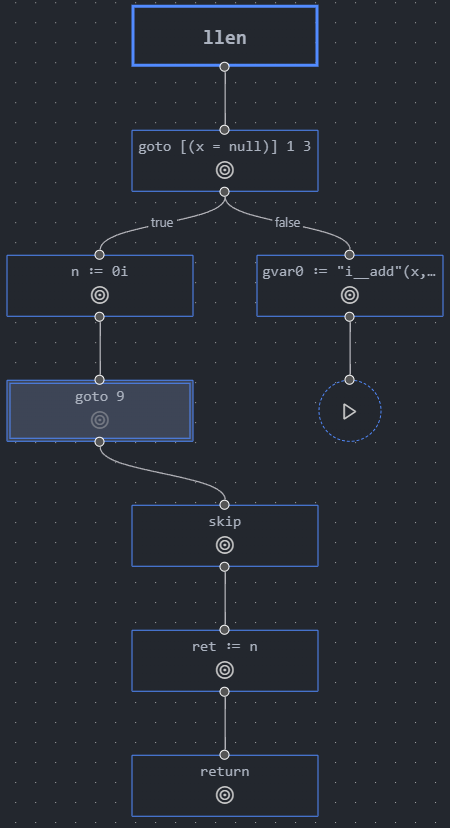
\includegraphics[width=0.75\textwidth]{img/execmap-init.png}
    \caption{The execution map of a partially completed symbolic execution}%
    \label{fig:execmap-init}
  \end{subfigure}
  \qquad
  \begin{subfigure}[b]{0.4\textwidth}
    \centering
    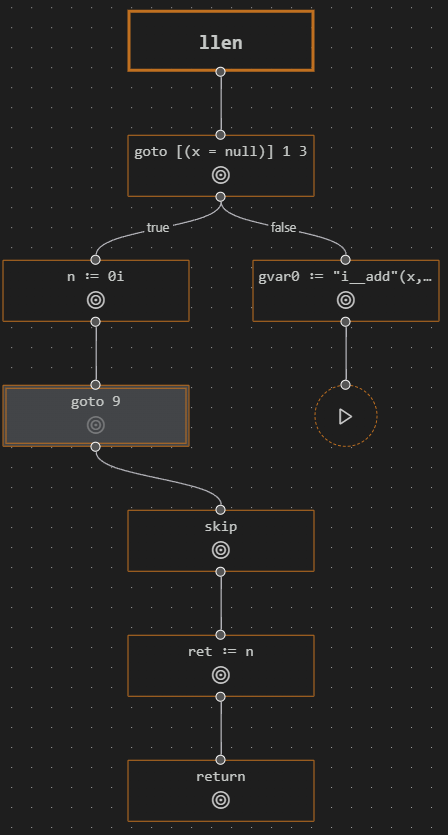
\includegraphics[width=0.75\textwidth]{img/execmap-theming.png}
    \caption{
      A demonstration of the interface adapting to the user's selected editor
      colour scheme}%
    \label{fig:execmap-theming}
  \end{subfigure}
  \caption{The first iteration of the exec map display}
\end{figure}

Next came the unification UI.\@ To prevent large amounts of code duplication,
much of the code for the exec map view component was refactored into the generic
\texttt{<TreeMapView />} component; this component handles setting up the React
Flow renderer, as well as recursively defining nodes from an execution or
unification map based on a function supplied via props, and rendering nodes
using a custom component (see \autoref{lst:treemapview-types} for the relevant
types). The exec map was extended with a badge that displays when a command has
a unification under it, and the result of that unification. When a command with
a unification is selected, the extension calls the \texttt{Unification\_command}
to load the relevant unify map, which is then displayed
(\autoref{fig:unifymap-init}) in a separate tab in the webview. When viewing
unification, a resizeable sidebar (courtesy of the Allotment
library~\cite{allotment}) with information on the selected assertion is
displayed (\autoref{fig:unifymap-sidebar}).

\begin{figure}
  \centering
  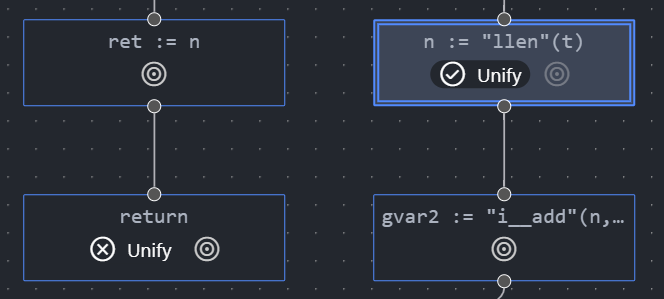
\includegraphics[width=0.5\textwidth]{img/execmap-unify.png}
  \caption{A demonstration of the Unify badge in the execution map}%
  \label{fig:execmap-unify}
\end{figure}

\begin{figure}
  \centering
  \begin{subfigure}[b]{0.3\textwidth}
    \centering
    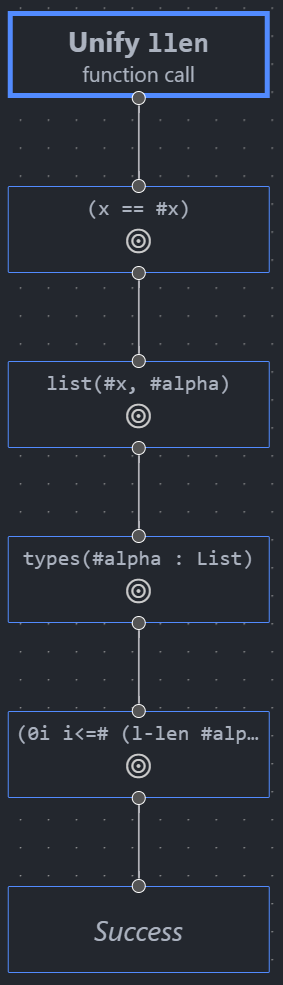
\includegraphics[width=0.6\textwidth]{img/unifymap-init.png}
    \caption{The unification map}%
    \label{fig:unifymap-init}
  \end{subfigure}
  \qquad
  \begin{subfigure}[b]{0.5\textwidth}
    \centering
    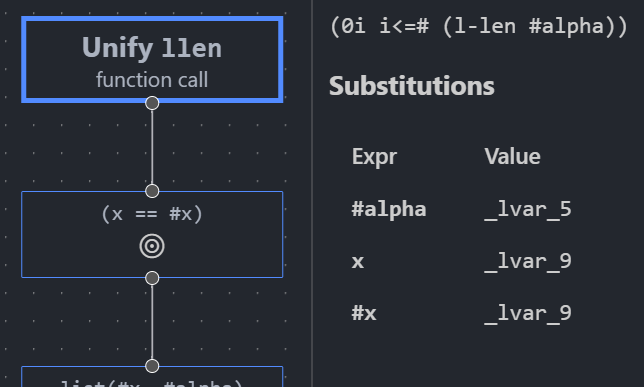
\includegraphics[width=0.75\textwidth]{img/unifymap-sidebar.png}
    \caption{The assertion data sidebar}%
    \label{fig:unifymap-sidebar}
  \end{subfigure}
  \caption{The first iteration of the unification map display}
\end{figure}

Of course, the top-level unification doesn't tell the full story --- displaying
folds is required for the complete picture. Similar to the exec map's unify
badges, an assertion node with a fold displays a fold badge. Once selected,
the data sidebar displays a button to `step in' to this fold
(\autoref{fig:unifymap-fold-button}). Internally, the webview effectively tracks
a stack of unification IDs, displaying the topmost unification in the
unification tab, and displaying breadcrumbs (\autoref{fig:unifymap-breadcrumbs})
in the data sidebar that can be used to instantly step back out as far as
desired.

\begin{figure}
  \centering
  \begin{subfigure}[b]{0.45\textwidth}
    \centering
    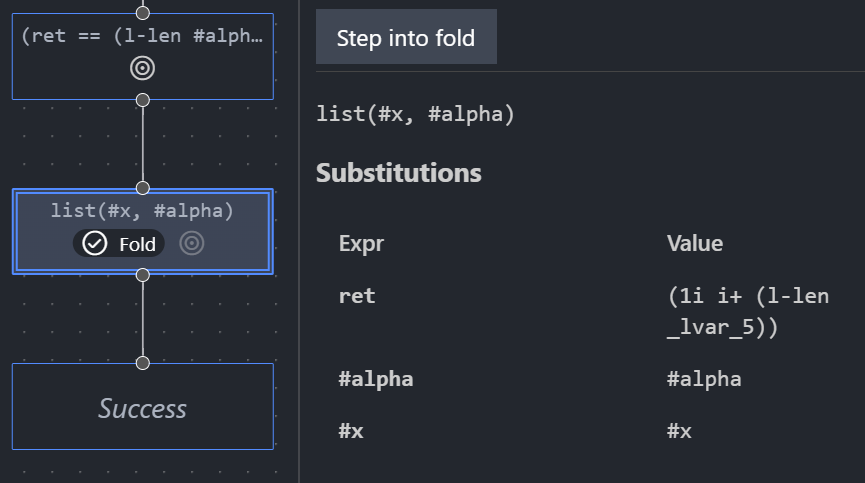
\includegraphics[width=\textwidth]{img/unifymap-fold-button.png}
    \caption{The button for stepping into a fold}%
    \label{fig:unifymap-fold-button}
  \end{subfigure}
  \quad
  \begin{subfigure}[b]{0.45\textwidth}
    \centering
    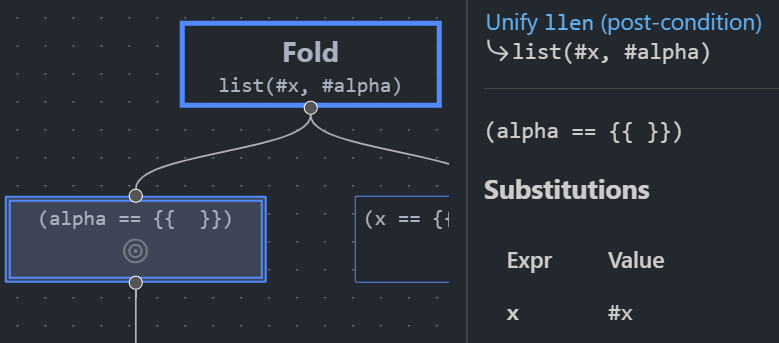
\includegraphics[width=\textwidth]{img/unifymap-breadcrumbs.png}
    \caption{The breadcrumbs used to step out of unification folds}%
    \label{fig:unifymap-breadcrumbs}
  \end{subfigure}
  \caption{UI elements concerning folds}
\end{figure}

While implementing the debug interface for GIL is a vast improvement upon
previous debugging methods, the ability to work with Gillian's functionality
to lift information to the target language would be much desired. While support
for this is partially implemented (\autoref{fig:execmap-wisl}), there are some
technical challenges that are outside the scope of this project, and are as yet
unsolved. The current implementation uses a secondary \texttt{ExecMap} to track
the execution map in the lifted context, containing references to the relevant
report IDs for execution of GIL commands, and serves that to the debug interface
instead of the base exec map if applicable. This solution isn't fully
functional: for example, a node for an if-else statement appears both before
and after the conditional block in the execution map, and debugger cannot
handle a situation in which a branching GIL command followed by other commands
are lifted to a single target language statement.

\begin{figure}
  \centering
  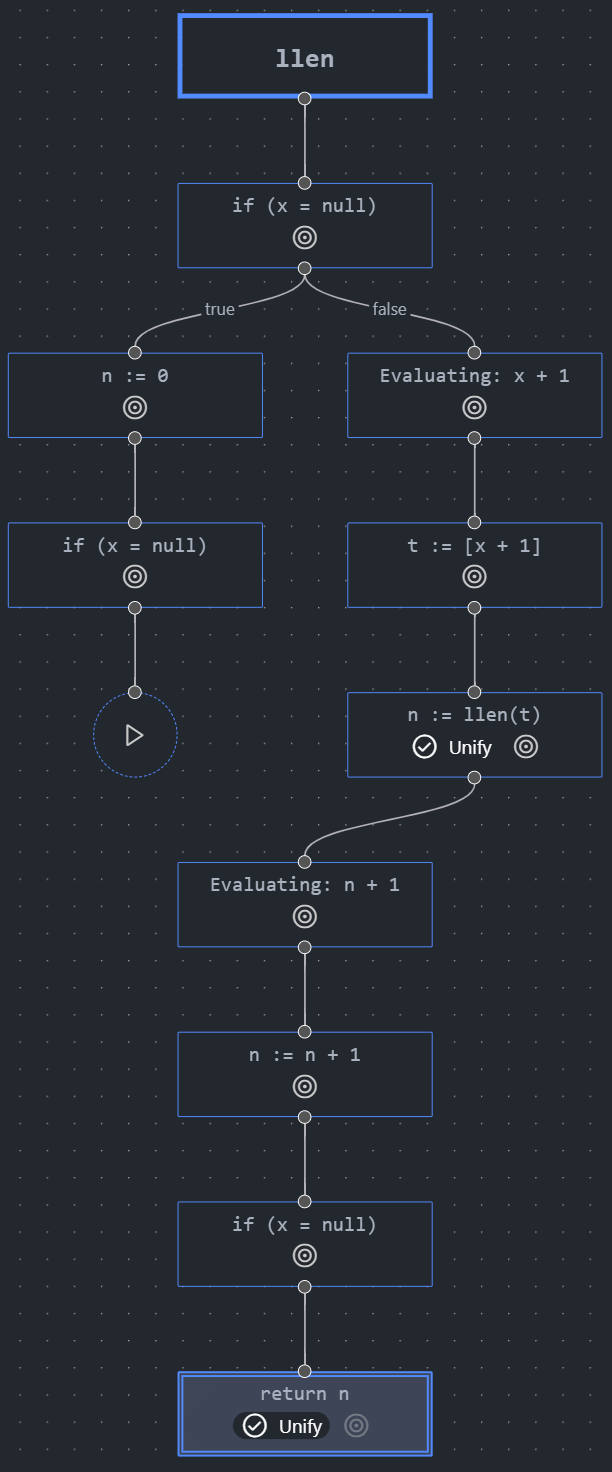
\includegraphics[width=0.35\textwidth]{img/execmap-wisl.png}
  \caption{A demonstration of partial support for WISL lifting in the debugger
  interface}%
  \label{fig:execmap-wisl}
\end{figure}
